\documentclass[11pt, twoside]{article}

\usepackage{graphicx}
\usepackage{amsmath, amssymb}
\usepackage{enumerate}
\usepackage{titleps}
\usepackage[top=1.25in,bottom=1in,right=1in,left=1in]{geometry}
\usepackage[parfill]{parskip}
\usepackage{titling}
\usepackage{hyperref}
\hypersetup{
    colorlinks=true,
    linkcolor=blue,
    filecolor=magenta,      
    urlcolor=cyan,
}

\graphicspath{ {../images/} }


\newpagestyle{ruled}
{\setfoot{}{\thepage}{} \footrule}
\pagestyle{ruled}


\setlength{\droptitle}{-4em}   % This is your set screw
\posttitle{\par\end{center}\vskip 0.5em}


\title{6.867 Project - Milestone 5}
\date{November 21st, 2017}
\author {Kimberly Villalobos Carballo, Timothy Leplae-Arthur, Sean Fraser}


\begin{document}
\maketitle

Since our previous milestone which stated our initial results, in addition to testing both our Edge Based CNN Segmentation and our clustering based method on more datapoints, we aimed to further analyze and compare these methods through various pre and post-processing techniques. In particular, to fine-tune our accuracies and results, we looked at pre-processing via image smoothing \cite{Xu}, transformations, and post-processing via edge thinning. 

\textbf{Edge Thinning:}

In this post processing technique, for the CNN, we first nullified those pixels whose value in the gray scale was below a certain threshold, and then we apply matlab morphological operations to thin the edges obtained from the output of the neural network. This technique removes pixels so that an object without holes shrinks to a minimally connected stroke, and an object with holes shrinks to a connected ring halfway between each hole and the outer boundary. As we can observe in the images above, the segmentation obtained after thinning the edges is much better than the one we had obtained for the last milestone.

\begin{figure}[ht]
    \centering
    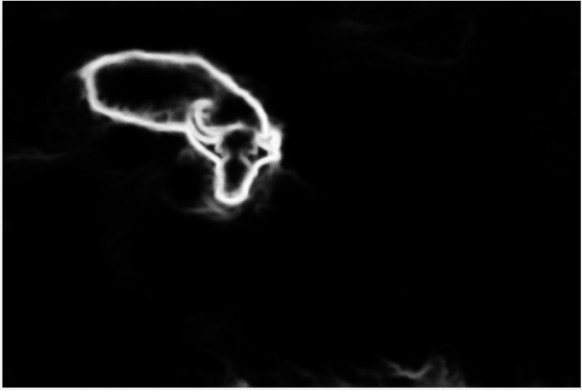
\includegraphics[width=1.5in]{thin1}
    
\includegraphics[width=1.5in]{thin2}
    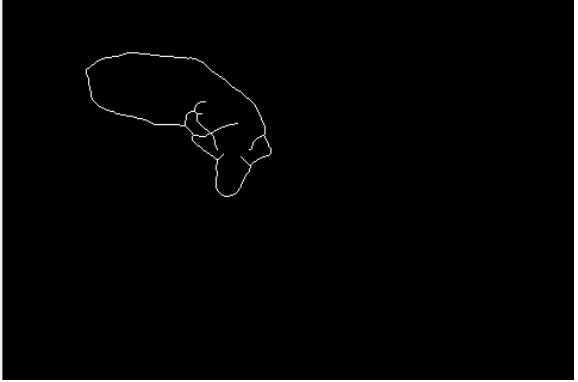
\includegraphics[width=1.5in]{thin3}
    
\includegraphics[width=1.5in]{thin4}    
    \includegraphics[width=1.5in]{thin7}
    \includegraphics[width=1.5in]{thin8}
    \includegraphics[width=1.5in]{thin5}
    \includegraphics[width=1.5in]{thin6}

    \caption{Comparison of the output edge map of the CNN (1st column), the segmentation based on that output with no post-processing (2nd column), the result of edge thinning on the edge map (3rd column), and finally the segmentation based on the thinner edge map after post-processing (4th column), for two images from the previous milestone}
    \label{fig:reg1}
\end{figure}


\textbf{Image Smoothing:}

For this pre-processing technique, we used the same procedure outlined in \cite{Xu}, that is Image Smoothing via $L_0$ Gradient Minimization. This algorithm aims to reduce the complexity/ noise of the natural images. This method seems to have improved the accuracies of the segmentations for our K-means clustering based method but seems to have made little or no difference with the CNN based method. This is what we expect, as the clustering approach is fairly primitive, so adding this extra layer of processing helps, whereas in the CNN, this may already be handled in some way through the convolutional or pooling layers of the network architecture. 

For our clustering based approached we obtained the following results:

\begin{figure}[ht]
    \centering
    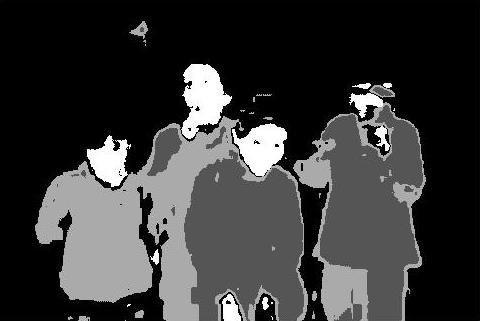
\includegraphics[width=1.5in]{290035_k4_l0}
    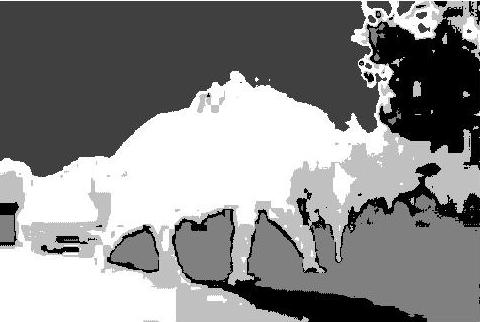
\includegraphics[width=1.5in]{296028_k5_l0}
    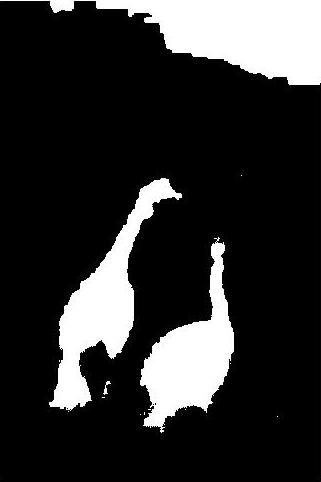
\includegraphics[width=0.9in]{289011_k2_l0}    
    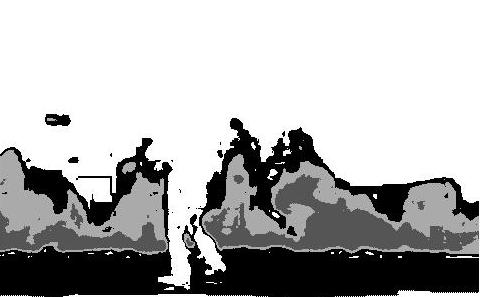
\includegraphics[width=1.5in]{285022_k4_l0}
    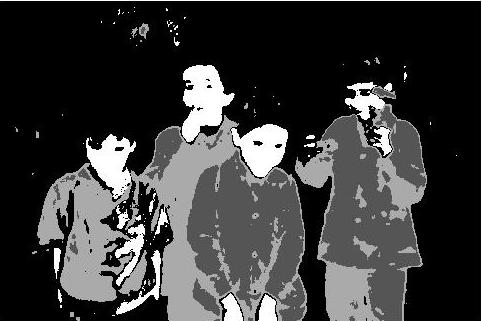
\includegraphics[width=1.5in]{290035_k4}
    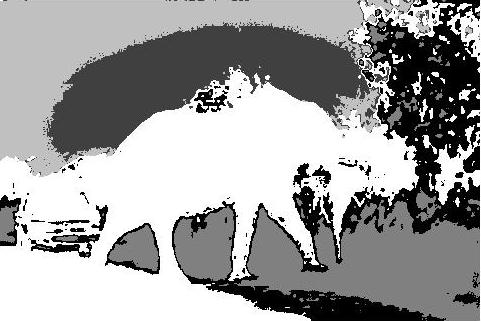
\includegraphics[width=1.5in]{296028_k5}
    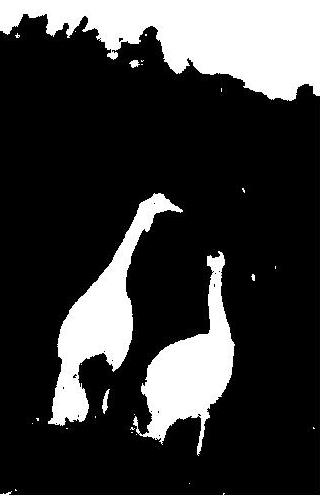
\includegraphics[width=0.9in]{289011_k2}
    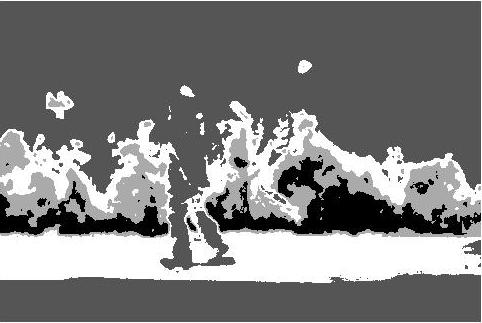
\includegraphics[width=1.5in]{285022_k4}

    \caption{Results of Image Smoothing on our clustering on four different images. The first row shows results of the clustering algorithm after image smoothing / denoising. The second row is the result of the clutering on original image. }
    \label{fig:reg3}
\end{figure}

As we can see, for some images, like the first one, it greatly improves the clustering, while for more complicated images like the last one, it is hard to see the improvements. 

For the neural network we obtained the following results: 

\begin{figure}[ht]
    \centering
    \includegraphics[width=2.0in]{orig1}
    \includegraphics[width=2.0in]{smooth1}
    \includegraphics[width=2.0in]{gt1}
    \includegraphics[width=2.0in]{orig2}
    \includegraphics[width=2.0in]{smooth2}
    \includegraphics[width=2.0in]{gt2}

    \caption{Results of Image Smoothing on our CNN based approach. The first row shows the output segmentations, while the second row shows the output edge maps. The first column is the output of the CNN based on the original image, the second column is the output from the image pre-processed via image smoothing, and the thrid columnd is the ground truth output.}
    \label{fig:reg2}
\end{figure}

\textbf{Transformations:}

Finally, we tried 7 different transformations of the input images to check if our segmentation results improved. For the NN approach, we can see in the images below that changing the contrast and brightness of the images helped obtain better defined edges that resulted in better segmentations. For instance, increasing the contrast helped our algorithm find the path and the car in the image.


\begin{figure}[ht]
    \centering
    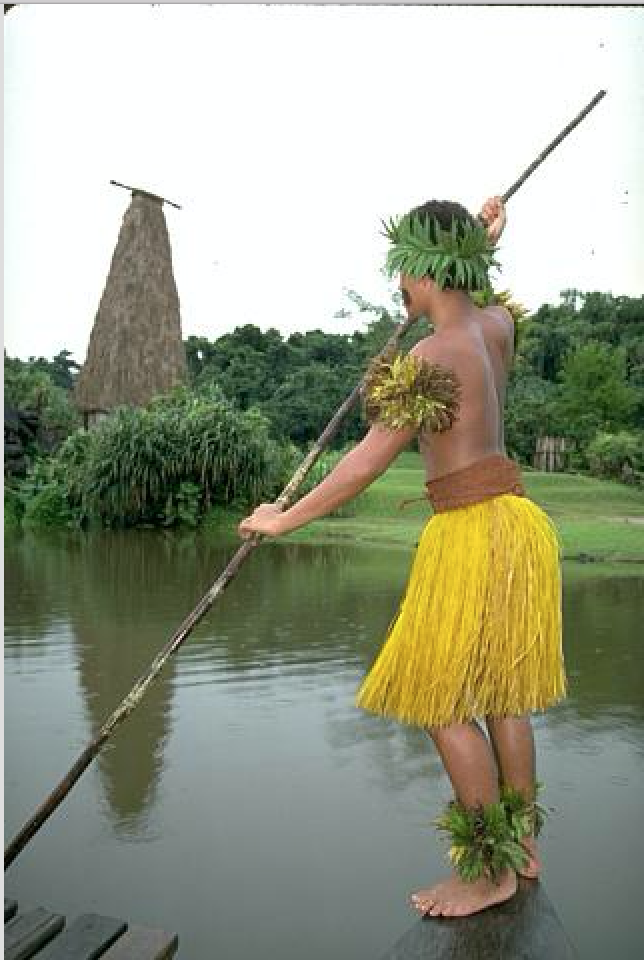
\includegraphics[width=1.5in]{original}
    \includegraphics[width=1.5in]{T1}
    \includegraphics[width=1.5in]{T2}
    \includegraphics[width=1.5in]{T3}
    \includegraphics[width=1.5in]{T4}
    \includegraphics[width=1.5in]{T5}
    \includegraphics[width=1.5in]{T6}
    \includegraphics[width=1.5in]{T7}

    \caption{Segmentation results for the following transformations for the NN: original, gray-scale, increase sharpness, blur image, low contrast, high contrast, dark image, high brightness (from left to right, top to bottom)}
    \label{fig:reg4}
\end{figure}

\newpage
\begin{thebibliography}{9}
\bibitem{Arbelaez}
Arbelaez, P.; Maire, M.; Fowlkes, C.; Malik, J. (2011)
``Contour Detection and Hierarchical Image Segmentation"
\textit{IEEE TPAMI} 33.5: 898-916
\bibitem{El-Sayed}
El-Sayed, M.; Estaitia, Y.; Khafagy M. (2013)
``Automated Edge Detection Using Convolutional
Neural Network"
\textit{International Journal of Advanced Computer Science and Applications} 4.10
\bibitem{Xu}
Xu, L.; Lu, C.; Xu, Y.; Jia, J. (2011)
``Image Smoothing via $L_0$
 Gradient Minimization"
\textit{ACM Trans. Graph.} 30.6
\bibitem{Kaur}
Kaur, D.; Kaur, Y. (2014)
``Various Image Segmentation
Techniques: A Review"
\textit{International Journal of Computer Science and Mobile Computing} 3.5: 809-814
\bibitem{Wang}
Wang, R. (2016)
``Edge Detection Using Convolution Neural Network"
\textit{Advances in Neural Networks - ISNN} 20: 741
\end{thebibliography}

\end{document}